\begin{exercises} 

\item What is the formula for a sinusoidal function that has a minimum at coordinates
    $(3,6)$ followed by a maximum at $(5,9)$?  %  1.5 \sin(\frac{ \pi}{2} (x-3)) + 7.5 
\begin{exerciseSolution}
\end{exerciseSolution}


\item If we take a sinusoidal function $f(t)= A \sin ( B (t - t_0)) + C$ and replace one of
    the parameters with a another function, say a linear function, we can create more
    complicated shapes.  Find formulas for the function plotted in the following graphs.

    \def\scl{0.9}
    \begin{center}
        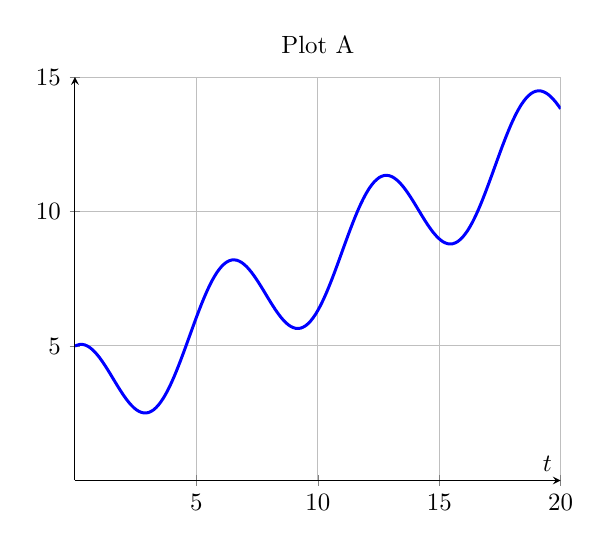
\begin{tikzpicture}[scale=\scl]
            \begin{axis}[axis lines=center, xmin=0, xmax=20, ymin=0, ymax=15, domain=0:20,
                xlabel={$t$}, title={Plot A}, grid]
                \addplot[smooth, blue, very thick, samples=100] {2*cos(deg(x)) + 3 + 0.5*x};
            \end{axis}
        \end{tikzpicture}
        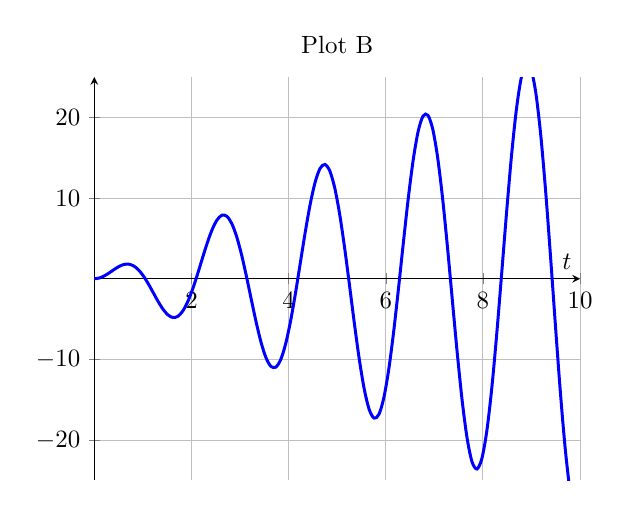
\begin{tikzpicture}[scale=\scl]
            \begin{axis}[axis lines=center, xmin=0, xmax=10, ymin=-25, ymax=25, domain=0:10,
                xlabel={$t$}, title={Plot B}, grid]
                \addplot[smooth, blue, very thick, samples=100] {3*x*sin(deg(3*x))};
            \end{axis}
        \end{tikzpicture}
        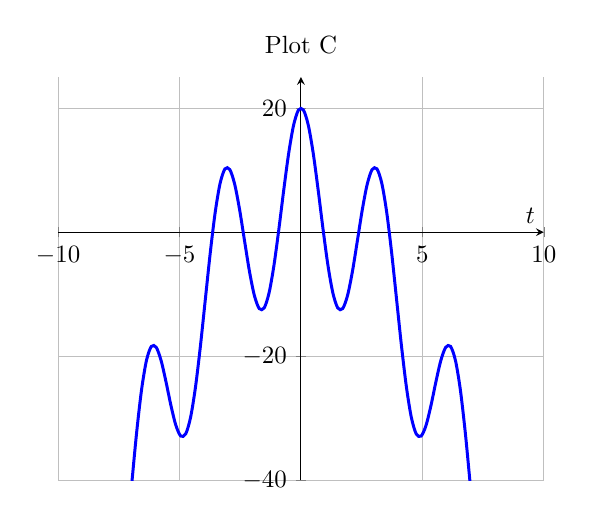
\begin{tikzpicture}[scale=\scl]
            \begin{axis}[axis lines=center, xmin=-10, xmax=10, ymin=-40, ymax=25, domain=-10:10,
                xlabel={$t$}, title={Plot C}, grid]
                \addplot[smooth, blue, very thick, samples=100] {15*cos(deg(2*x))+5-x^2};
            \end{axis}
        \end{tikzpicture}
        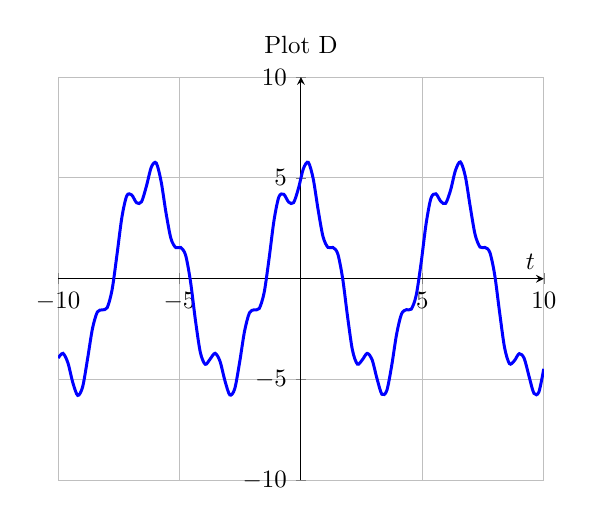
\begin{tikzpicture}[scale=\scl]
            \begin{axis}[axis lines=center, xmin=-10, xmax=10, ymin=-10, ymax=10, domain=-10:10,
                xlabel={$t$}, title={Plot D}, grid]
                \addplot[smooth, blue, very thick, samples=100]
                {5*cos(deg(x))+1*sin(deg(5*x))};
            \end{axis}
        \end{tikzpicture}
    \end{center}
\begin{exerciseSolution}
    \ba
        \item $f(t) = 2\cos(t) + 3 + 0.5*t$ over the range $[0,20]$
        \item $f(t) = 3t \sin(3t)$ over the range $[0,10]$
        \item $f(t) = 15\cos(2t) + 5-t^2$ over $[-10,10]$
        \item $f(t) = 5\cos(t) + \sin(5t)$
    \ea
\end{exerciseSolution}


\item The number of hours of daylight varies sinusoidally throughout the year.  The
    maximum occurs on the summer solstice, June 21, when we have 15 hours and 50 minutes
    of daylight.  The minimum occurs on the winter solstice, December 21, when we have
    only 8 hours and 33 minutes of daylight.  Find the formula for a function to describe
    this.  The input to your function should be $d$, the number of days since the
    beginning of the year, so that $d = 5$ on January 5.  The output of your function
    should be the amount of daylight, in minutes.  Assume that this is not a leap year.
    Hint:  Because we know the date of maximum, it is easier to write this in terms of a
    cosine function.
    % f(d) = 218.5 cos( \frac{2 \pi}{365} (d – 172) ) + 731.5

\begin{exerciseSolution}
\end{exerciseSolution}



\end{exercises}
\afterexercises
